\documentclass[danish]{article}
\usepackage[utf8]{inputenc}
\usepackage[danish]{babel}
\usepackage[T1]{fontenc}	
\usepackage[a4paper, , margin=1in]{geometry}

\usepackage[framed,numbered,autolinebreaks,useliterate]{mcode} %matlab
\usepackage[version=3]{mhchem} % Package for chemical equation typesetting
\usepackage{siunitx} % Provides the \SI{}{} and \si{} command for typesetting SI units
\usepackage{graphicx} % Required for the inclusion of images
\usepackage{subcaption} % Add the possibility for subfigures/subcaptions.
\usepackage{natbib} % Required to change bibliography style to APA
\usepackage{amsmath} % Required for some math elements
\usepackage{amssymb}
\usepackage{float}
\graphicspath{ {graphics/} }
\setcounter{tocdepth}{1}
\setlength\parindent{0pt} % Removes all indentation from paragraphs

\renewcommand{\labelenumi}{\alph{enumi}.} % Make numbering in the enumerate environment by letter rather than number (e.g. section 6)
\begin{document}

\title{\textbf{Introduktion til Digital Signalanalyse }   Eksamensforberedelse}
\author{Jonas Lind}
\date{15-08-2017}
\maketitle
\tableofcontents
\newpage
\section{Analyse af digitale signaler med Diskret Fourier Transformation og Spektrogram}
\subsection{DFT}
\begin{itemize}
	\item Tidsinvariant (amplitude, frekvens og fase ændrer sig ikke med tiden indenfor vinduet der analyseres).
	\item Bruges til at transformere tidsdomæne data til frekvensdomæne data.
	\begin{itemize}
		\item Et tidsdiskret signal i tidsdomænet transformeres til et signal angivet som et komplekst frekvensspektrum i frekvensdomænet.
	\end{itemize}
\end{itemize}

\begin{equation}
X(m)=\sum_{n=0}^{N-1}x(n)e^{\frac{-j2\pi mn}{N}}
\end{equation}

{\setlength\parindent{24pt} $n$ = tidsindex, $m$ = frekvensindex, $f_s$ = samplingsfrekvens, $N$ = antal samples}

\begin{itemize}
	\item Eulers formel bruges for at beregne den reelle del og den imaginære del.
\end{itemize}

\begin{equation}
e^{-j\theta}=\cos(\theta) -j\sin(\theta)
\end{equation}

\begin{equation}
X(m)=\sum_{n=0}^{N-1}x(n)(\cos{\left(\frac{-j2\pi mn}{N}\right)}\sin{\left(\frac{-j2\pi mn}{N}\right)})
\end{equation}

\paragraph{Amplitudespektrum} Amplituden af X(m) kan beregnes ved længden af den reelle og imaginære del.

\begin{equation}
|X(m)|=\sqrt{Re(X(m))^2+Im(X(m))^2}
\end{equation}

\paragraph{Effektspektrum} Effekten af X(m) kan beregnes ved at opløfte amplituden i 2. potens. 

\begin{equation}
|X(m)|^2
\end{equation}

\paragraph{Analyse frekvens} Samplefrekvensen kan findes ved en sample periode.

\begin{equation}
f_s=\frac{1}{t_s}
\end{equation}

\begin{equation}
f_{analyse}(m)=\frac{m f_s}{N}
\end{equation}

\subsection{Frekvensopløsning}
	\begin{itemize}
	\item Længden af vinduet bestemmer frekvensopløsningen.
­	\begin{itemize}
	\item Et bredt vindue øger frekvens opløsningen, men der ting der forhindrer det praktisk.
	\item Hvis ikke $\Delta R$ går op i sinus signalet kommer der spektral forbredning.
\end{itemize} 
	\item Inputsignalet har en frekvens der ligger under $\Delta R$, vil der opstå spektral forbredning og inputsignalet vil vise sig i alle output "bins".
\end{itemize}

\begin{equation}
\Delta R = \frac{f_s}{N}
\end{equation}

\begin{itemize}
	\item Et bredt vindue medfører
­	\begin{itemize}
	\item Sampletiden forlænges og det betyder lange delays og en større DFT udregning.
­	\item Et langt vindue vil resultere i et signal der varierer med tiden.
­	\item Det medfører en ukorrekt frekvensanalyse hvis DFT udføres på et signal der ændrer sig over tid.
	\end{itemize}
\end{itemize}

\subsection{Short-Time DFT} 
\begin{itemize}
	\item Løsningen på at udføre DFT på et bredt vindue.
­	\begin{itemize}
	\item Bryder et langt signal ned til mindre segmenter og analysere hvert enkelt segment med DFT.
­	\item Segmenterne er i et fast interval fra $k = 0$ til $k = N-1$.
­	\item Når n ændres glider vinduet over på et andet segment af signalet. 
\end{itemize}
\end{itemize}

\subsection{Spektrogram}
\begin{itemize}
	\item Der er et trade-off imellem en god frekvensopløsning eller en god tidsopløsning. 
­	\begin{itemize}
		\item Et smalt vindue giver en god opløsning i tid, men giver en dårlig opløsning i frekvens. 
­		\item Et bredt vindue giver en god opløsning i frekvens, men en dårlig opløsning i tid. 
	\end{itemize}
\end{itemize}

\begin{figure}[H]
	\centering
	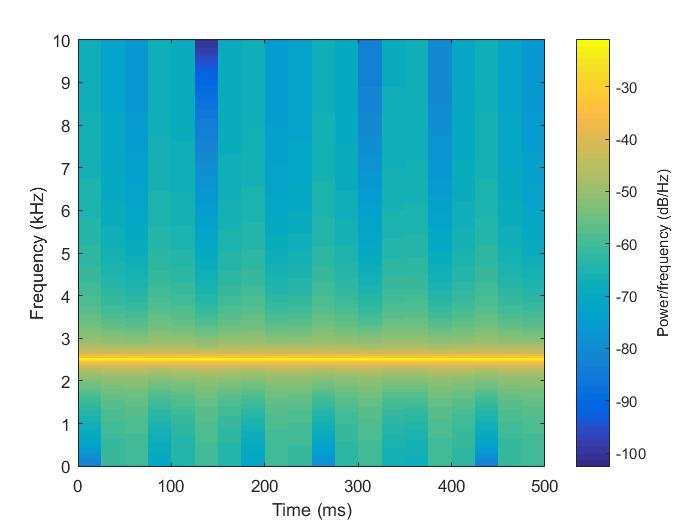
\includegraphics[width=0.6\linewidth]{graphics/spectrogram}
	\caption{Spektrogram af frekvenserne sendt gennem kommunikationssystemet Frequency-Shift Keying.}
	\label{fig:spectrogram}
\end{figure}

\subsection{Invers-DFT}
\begin{itemize}
	\item Bruges til at transformere frekvensdomæne data til tidsdomæne data.
\end{itemize}

\begin{equation}
X(m)=\frac{1}{N}\sum_{m=0}^{N-1}X(m)e^{\frac{j2\pi mn}{N}}
\end{equation}



\newpage
\section{Spektral forbredning, zero-padding og window functions i relation til DFT}
\subsection{DFT}
\begin{itemize}
	\item Tidsinvariant (amplitude, frekvens og fase ændrer sig ikke med tiden indenfor vinduet der analyseres).
	\item Bruges til at transformere tidsdomæne data til frekvensdomæne data.
	\begin{itemize}
		\item Et tidsdiskret signal i tidsdomænet transformeres til et signal angivet som et komplekst frekvensspektrum i frekvensdomænet.
	\end{itemize}
\end{itemize}

\begin{equation}
X(m)=\sum_{n=0}^{N-1}x(n)e^{\frac{-j2\pi mn}{N}}
\end{equation}

\subsection{Spektral forbredning}
\begin{itemize}
	\item Længden N af vinduet bestemmer frekvensopløsningen.
	\item Et bredt vindue øger frekvens opløsningen, men der er ting der forhindrer det praktisk.
\end{itemize}

\begin{equation}
\Delta R=\frac{f_s}{N}
\end{equation}

\begin{itemize}
	\item Hvis ikke $\Delta R$ går op i sinus signalet kommer der spektral forbredning. 
	\begin{itemize}
		\item Inputsignalet har en frekvens der ligger mellem vores analyse frekvenser hvorved der opstår spektral forbredning og inputsignalet vil vise sig i alle output "bins" = $m$.
	\end{itemize}
\end{itemize}

\begin{equation}
f_{analyse}(m)=\frac{m f_s}{N}
\end{equation}

\begin{itemize}
	\item Antal samples N er invers proportional med hovedsløjfens (main lobe) bredde.
	\item Spektral forbredning kan nemmere ses på en decibel skala.
\end{itemize}

\begin{figure}[H]
	\centering
	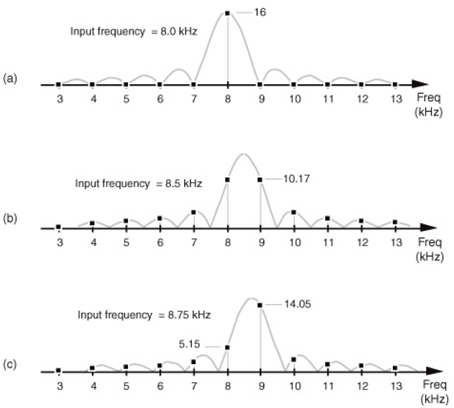
\includegraphics[width=0.6\linewidth]{graphics/leakage}
	\caption{Spektral forbredning.}
	\label{fig:leakage}
\end{figure}

\subsection{Zero-padding}
\begin{itemize}
	\item Ved zero-padding forlænges et signal ved at tilføje et n antal 0'er til det oprindelige signal. 
	\item Dette er med til at øge antallet af samples N også kaldet bins i frekvensdomænet, hvilket forbedrer frekvensopløsningen på signalet.
	\item Når der anvendes zero-padding skal det gøres før der foretages frekvensanalyse med DFT.
\end{itemize}

\begin{figure}[H]
	\centering
	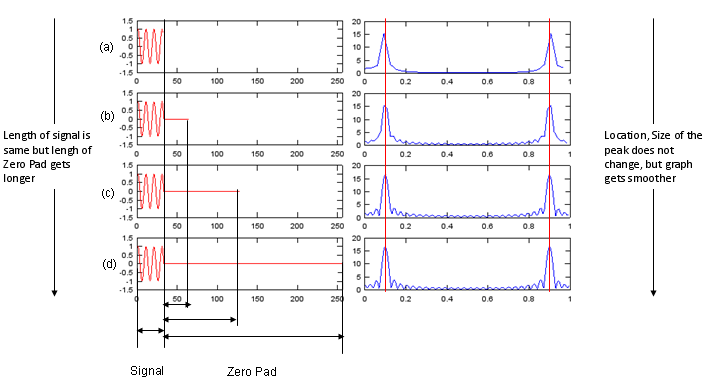
\includegraphics[width=0.8\linewidth]{graphics/zeropadding}
	\caption{Zeropadding (a) N = 16, (b) N = 32, (c) N = 64, (d) N = 128.}
	\label{fig:zeropadding}
\end{figure}

\subsection{Window functions}
\begin{itemize}
	\item Vindues metoder reducerer DFT-lækage ved at minimere størrelsen af sinc-funktionens sidelobes.
­	\begin{itemize}
		\item 	Samme amplitudeværdi af inputtet ved både start og slutningen af sample intervallet. 
­		\item Hovedsløjfens peak værdi reduceres – kaldes for processing loss of a window. 
	\end{itemize}
	\item Tradeoff
­	\begin{itemize}
		\item 	Bredden af hovedsløjfen, dæmpningen af sidesløjferne og hastigheden hvorved de dæmpes.
	\end{itemize}
	\item Anvendelse af både zerro-padding og window functions
­	\begin{itemize}
		\item Vinduesfunktionen må kun anvendes på det originale signal inden der foretages zerro-padding.
	\end{itemize}
\end{itemize}

\begin{figure}[H]
	\centering
	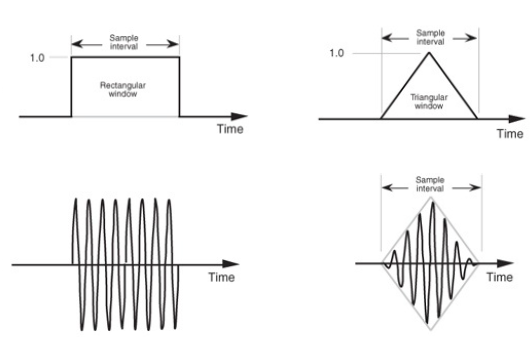
\includegraphics[width=0.6\linewidth]{graphics/windows}
	\caption{Rektangulær og Triangulær vinduesfunktion.}
	\label{fig:windows}
\end{figure}

\newpage
\section{FIR/IIR filter analyse og design vha. placering af poler/nuller i pol-nulpunkts-diagrammet}

\subsection{FIR- og IIR-filtre generelt}
\begin{itemize} 
	\item FIR filter output samples afhænger kun af tidligere input samples.
	\item IIR filter output samples afhænger af tidligere input samples og af tidligere  output samples.
	\item FIR filter har et endeligt impuls-respons og $h(n)$ = filter-koefficienter.
	\item IIR filter har et uendeligt impuls-respons og $h(n)$ skal med tiden falde mod 0 for at det er stabilt. 
\end{itemize}

\begin{figure}[H]
	\centering
	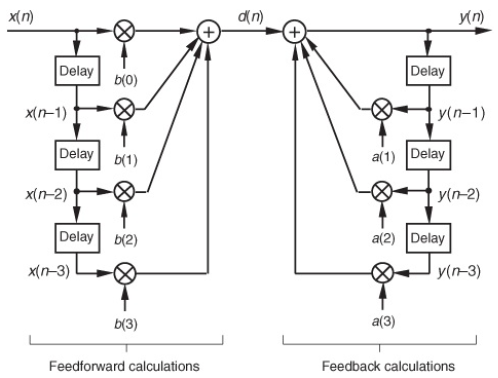
\includegraphics[width=0.6\linewidth]{graphics/iir}
	\caption{IIR digital filter struktur med feedforward og feedback udregninger.}
	\label{fig:iir}
\end{figure}

Differensligning - Finite Impulse Response (FIR)
\begin{equation}
y(n) = b_0 x(n) + b_1 x(n-1) + ... + b_M x(n-M)
\end{equation}

Differensligning - Infinite Impulse Respons (IIR)
\begin{equation}
y(n) = b_0 x(n) + b_1 x(n-1) + ... + b_M x(n-M) + a_1 y(n-1) + a_2 y(n-2) + ... + a_N y(n-N)
\end{equation}

\begin{itemize}
	\item Filtrets orden er største værdi af N og M.
\end{itemize}

\subsection{Pol-nulpunkts analyse}
\begin{itemize}
	\item FIR eller IIR-filter?
	\begin{itemize}
		\item FIR har kun poler i origo.
		\item IIR har flere poler.
	\end{itemize}
	\item Poler danner peaks.
	\begin{itemize}
		\item Har betydning for hvor meget frekvenserne bliver forstærket, hvis den placeres på enhedscirklen forstærkes frekvenserne uendeligt meget.
	\end{itemize}
	\item Nulpunkter danner dyk.
	\begin{itemize}
		\item Har betydning for hvor meget frekvenserne bliver dæmpet, hvis den placeres på enhedscirklen dæmpes frekvenserne uendeligt meget.
	\end{itemize}
\end{itemize}

\begin{figure}[H]
	\centering
	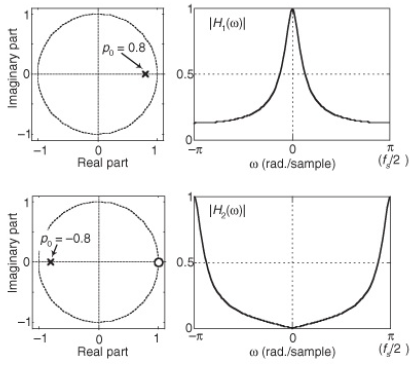
\includegraphics[width=0.4\linewidth]{graphics/iir_pz1}
	\caption{IIR filter poler/nulpunkter og normaliseret frekvens respons.}
	\label{fig:iir_pz1}
\end{figure}

\begin{figure}[H]
	\centering
	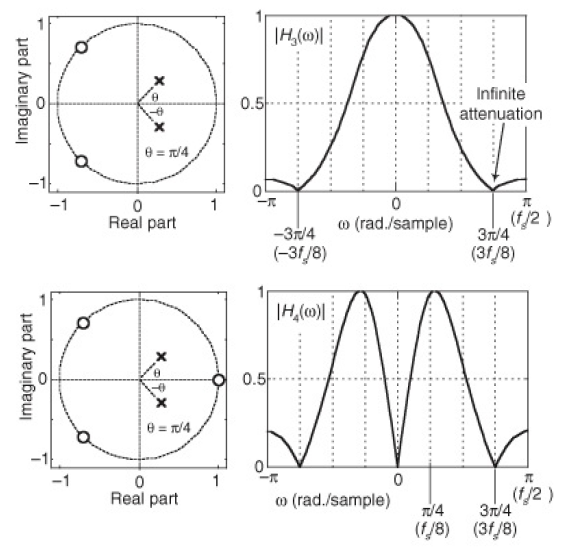
\includegraphics[width=0.4\linewidth]{graphics/iir_pz2}
	\caption{IIR filter poler/nulpunkter og normaliseret frekvens respons.}
	\label{fig:iir_pz2}
\end{figure}

\begin{itemize}
	\item Stabilitet.
	\begin{itemize}
		\item Hvis alle poler er placeret inde i enhedscirklen vil filteret være stabilt.
		\item Polen kan ophæves ved at have et nulpunkt med præcis samme afstand fra (0,0) og dermed samme længde.
		\item Poler/nulpunkter placeret i (0,0) påvirker ikke filterets frekvens respons. 
	\end{itemize}
\end{itemize}

\begin{figure}[H]
	\centering
	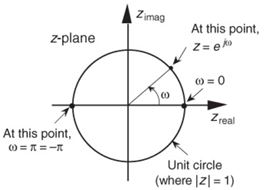
\includegraphics[width=0.8\linewidth]{graphics/unitycircle}
	\caption{s-planet og z-planet.}
	\label{fig:unitycircle}
\end{figure}

\subsection{Design af 2. ordens IIR filter}
\begin{itemize}
	\item Et 2. ordens IIR notch filter designes ved at placere poler og nulpunkter i z-domænet.
	\item Nulpunkter/poler har en radius og vinkel da de er komplekse tal.
	\begin{itemize}
		\item $r$ er nul-radius og $\omega$ er nul-vinkel.
		\item Nul-radius sættes til 1 og pol-radius sættes til 0,9 da det et skarpt filter ønskes.
	\end{itemize}
\end{itemize}

\begin{equation}
z_0 = r e^{j\omega} \mid p_0 = r e^{j\omega}
\end{equation}

\begin{itemize}
	\item Vinklen af de to nulpunkter og to poler beregnes (kompleks konjugerede).
\end{itemize}

\begin{equation}
\omega = 2\pi \frac{f}{f_s}
\end{equation}

\begin{figure}[H]
	\centering
	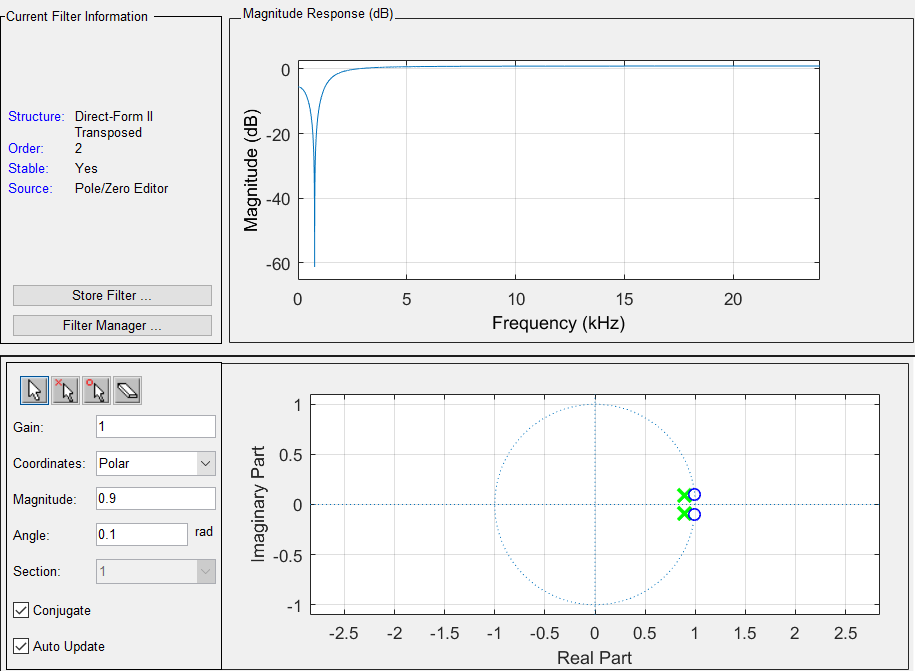
\includegraphics[width=0.6\linewidth]{graphics/notchfilter}
	\caption{Filter Designer tool i Matlab.}
	\label{fig:notchfilter}
\end{figure}

\begin{itemize}
	\item Overførelsesfunktionen H(z) i z-domænet opstilles ud fra poler/nulpunkter.
\end{itemize}

{\setlength\parindent{24pt}
\begin{tabular}{l}
	$z_0 =  e^{j0,1028}$ \\ 
	
	$\overline{z_0} =  e^{-j0,1028}$ \\ 
	
	$p_0 = 0,9 e^{j0,1028}$ \\ 
	
	$ \overline{p_0} = 0,9 e^{-j0,1028}$ \\ 
\end{tabular}} 

\begin{equation}
H(z) = \frac{Y(z)}{X(z)} = G \frac{(z - z_0)(z-\overline{z_0})}{(z - p_0)(z-\overline{p_0})} = G \frac{(z - e^{j0,1028})(z - e^{-j0,1028})}{(z - 0,9\cdot  e^{j0,1028})(z-0,9\cdot e^{-j0,1028})}
\end{equation}

\begin{figure}[H]
	\centering
	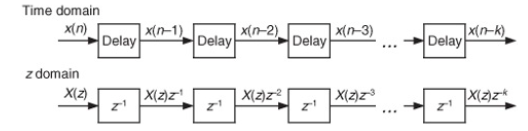
\includegraphics[width=0.6\linewidth]{graphics/z_domain_delay}
	\caption{Tids- og z-domæne delay.}
	\label{fig:z_domain_delay}
\end{figure}

\begin{itemize}
	\item Overførselsfunktionen H(z) skrives om således at polynomierne er opløftet negativt.
\end{itemize}

\begin{equation}
H(z) = \frac{z^2 - 1,99z + 0,99}{z^2 - 1,79z + 0,81} \cdot \frac{z^{-2}}{z^{-2}} \longrightarrow \frac{1 - 1,99z^{-1} + 0,99z^{-2}}{1 - 1,79z^{-1} + 0,81z^{-2}}
\end{equation}

\begin{itemize}
	\item Brøkerne kan skrives ud.
\end{itemize}

\begin{equation}
Y(z)(1-1,79z^{-1}+0,81z^{-2}) = X(z)(1-1,99z^{-1}+0,99 z^{-2})
\end{equation}

\begin{itemize}
	\item Differensligningen kan opstilles ved at anvende invers z-transformation.
\end{itemize}

\begin{equation}
y(n)-1,79y(n-1)+0,81y(n-2)=x(n)-1,99x(n-1)+0,99x(n-2)
\end{equation}

\begin{equation}
y(n)=1x(n)-1,99x(n-1)+0,99x(n-2)+1,79y(n-1)-0,81y(n-2)
\end{equation}



\newpage
\section{Window method til FIR filter design}

\begin{itemize}
	\item Metode til design af FIR filtre, hvor man i frekvensdomænet vælger frekvenser man ønsker at fjerne.
	\item Der bruges vinduer for at undgå Gibbs fænomen, som er 'ører' på et firkantsignal.
\end{itemize}
\subsection{Filter design}
\begin{itemize}
	\item Fastlæg samplefrekvensen samt knækfrekvenser.
	\begin{itemize}
		\item Antallet af filterkoefficienter/filterorden.
	\end{itemize}
	\item Lav ideelt filter I frekvensdomænet.
	\begin{itemize}
		\item Antal af bins bestemmer hvor præcist man kan ramme de valgte knækfrekvenser.
		\item Giver et større group delay. 
	\end{itemize}
	\item Det ideelle filters overføringsfunktion konstrueres op til $\frac{f_s}{2}$, hvorefter det spejles omkring $\frac{f_s}{2}$ for at danne den fulde overføringsfunktion. 
\end{itemize}

$N = 32$\\
\newline Normeret cut-off frekvens: $f_{cut} = 0,2$\\
\newline Hvilket bin-nummer rammer tættest på cut-off frekvensen: $N_{cut} = \frac{f_{cut}}{2}\cdot N = 3,2 \approx 3$\\

\begin{figure}[H]
	\centering
	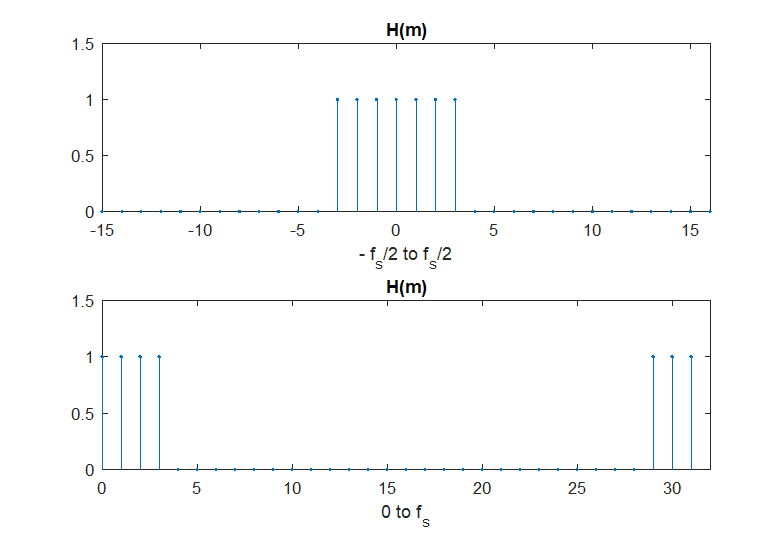
\includegraphics[width=0.6\linewidth]{graphics/windowmethod_1}
	\caption{Ideelt lavpasfilter set med kontinuert frekvensrespons og diskret frekvensrespons.}
	\label{fig:windowmethod_1}
\end{figure}

\begin{itemize}
	\item Der foretages en IDFT for at få filteret over i tidsdomænet.
	\begin{itemize}
		\item I tidsdomænet bliver responset repræsenteret som en sinc-funktion.
	\end{itemize}
	\item Sinc funktionen shiftes for at få peaket til at ligge midt i de valgte filterkoefficienter, da filterkoefficienterne skal være symmetriske for at få lineær fase.
	\begin{itemize}
		\item Den sidste sample fjernes for at shifte impulsresponsen.
	\end{itemize}
\end{itemize}

\begin{figure}[H]
	\centering
	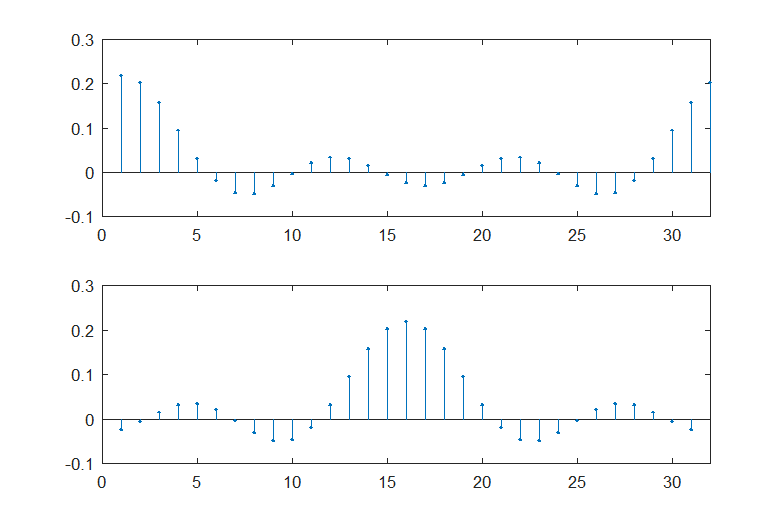
\includegraphics[width=0.6\linewidth]{graphics/windowmethod_2}
	\caption{IDFT af det diskrete respons efterfulgt af et symmetrisk respons der er blevet shiftet.}
	\label{fig:windowmethod_2}
\end{figure}

\begin{itemize}
	\item Et vindue ganges på for at udvælge betydende filterkoefficienter.
	\begin{itemize}
		\item Et vindue giver en kraftigere dæmpning.
	\end{itemize}
	\item Filteret kan trækkes over i frekvensdomænet med en DFT, for at validere at der gør som ønsket.
\end{itemize}

\begin{figure}[H]
	\centering
	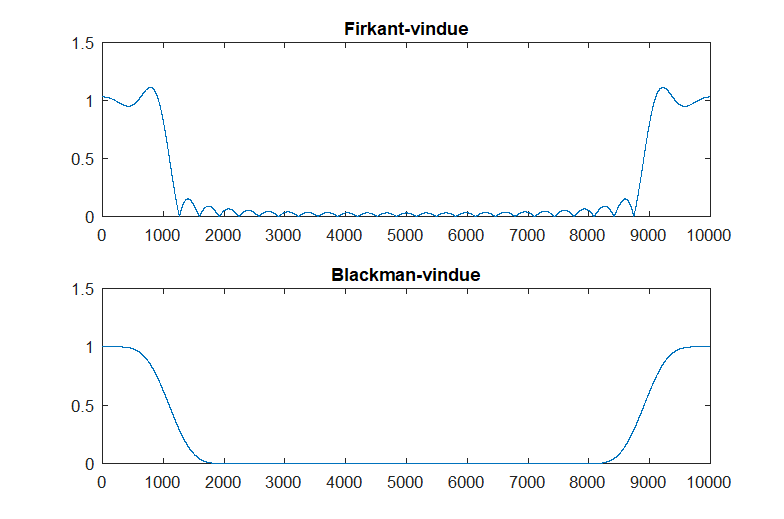
\includegraphics[width=0.6\linewidth]{graphics/windowmethod_3}
	\caption{Der anvendes DFT for at trække filteret over i frekvensdomænet for at validere det.}
	\label{fig:windowmethod_3}
\end{figure}

\subsection{Typer af vinduer}
\begin{itemize}
	\item Et firkant vindue giver den skarpeste cut-off frekvens, men resultere i ripple på flankerne.
	\begin{itemize}
		\item Skyldes at firkanten repræsenteres som en sinc i frekvensdomænet, som foldes med den ideelle overføringsfunktion.
	\end{itemize}
	\item Et Blackman vindue giver en større dæmpning og mindre ripple, men derimod mindre skarpe flanker.
\end{itemize}

\newpage
\section{Interpolation og decimation}
\subsection{Decimation}
\begin{itemize}
	\item To-trins proces med lavpasfiltrering efterfulgt af downsampling.
	\item Samplerate reduceres ved downsampling.
	\begin{itemize}
		\item En sekvens af samplede signalværdier kan downsamples med en faktor $M$ ved at beholde hver $M-$sample og kassere alle resterende samples.
	\end{itemize}
\end{itemize}

\begin{equation}
f_{s\, new} = \frac{f_{s\, old}}{M}
\end{equation}

\begin{equation}
x_{new}(m) = x_{old}(Mm)
\end{equation}

\begin{figure}[H]
	\centering
	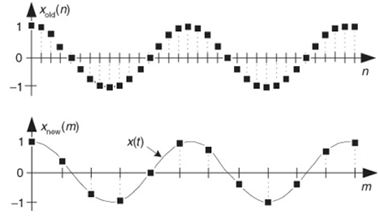
\includegraphics[width=0.6\linewidth]{graphics/decimation}
	\caption{Sample rate konvertering med den originale sekvens øverst og den downsampled med $M = 3$ sekvens nederst.}
	\label{fig:decimation}
\end{figure}

\begin{figure}[H]
	\centering
	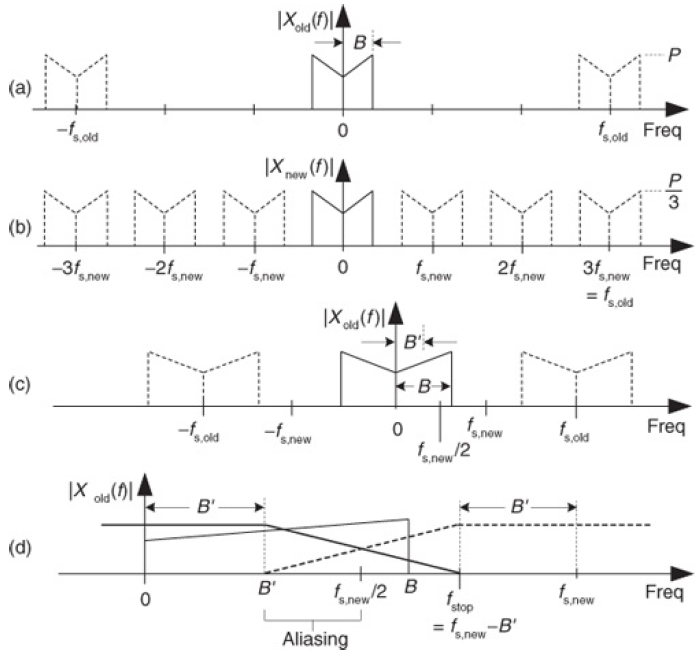
\includegraphics[width=0.6\linewidth]{graphics/decimation1}
	\caption{Spektrummet af et originalt båndbegrænset samplet $x_{old}(n)$ signal er indikeret med solid lines. Spektralreplikationerne er angivet med dashed lines.}
	\label{fig:decimation1}
\end{figure}

\begin{itemize}
	\item $X_{new}(f)$ kan være opnået direkte ved at sample det originale kontinuerlige $x(t)$ signal med en samplefrekvens på $f_{s\, new}$, i modsætning til nedsampling $x_{old}(n)$ med en faktor på tre.
	\item Der er en grænse for hvor meget der kan downsamples i forhold til båndbredden $B$ af det originale signal.
	\begin{itemize}
		\item 	Den nye samplefrekvens $f_{s\, new} > 2B$ for at forhindre aliasering.
		\item Hvis en decimation kræver $f_{s\, new} < 2B$, skal $x_{old}(n)$ være lavpasfiltreret før downsampling udføres.
		\begin{itemize}
			\item Hvis det originale signal har en båndbredde $B$ og det kun er båndbredden $B_v$ der er interessant at beholde skal signal spektrummet over $B'$ lavpas-filtreres med fuld dæmpning i stopbåndet fra $f_{stop}$.
			\item  Lavpas filteret's $f_{stop}$ frekvens kan være så høj som $f_{stop} = f_{s\,new} -B'$ og der vil ikke opstå aliasering i båndbredden $B'$.
		\end{itemize}
	\end{itemize}
		\item Downsampling medfører ikke amplitudetab i tidsdomænet.
		\item Downsampling medfører derimod et amplitudetab med en faktor $M$ i frekvensdomænet, $A_{new} = \frac{A}{M}$.
		\begin{itemize}
			\item DFT amplituden er proportional med antallet af samples i tidsdomænet.
		\end{itemize}
\end{itemize}

\begin{figure}[H]
	\centering
	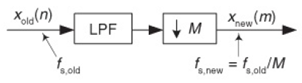
\includegraphics[width=0.4\linewidth]{graphics/decimation2}
	\caption{Decimation.}
	\label{fig:decimation2}
\end{figure}


\subsection{Interpolation}

\begin{itemize}
	\item Interpolation er en to-trins proces med upsampling efterfulgt af en lavpasfiltrering.
	\item Samplerate øges ved upsampling.
	\begin{itemize}
		\item 	For at øge samplefrekvensen $f_{s\, old}$ med en faktor $L$ indsættes $L-1$ zero-valued samples mellem hver sample i $x_{old}(n)$, hvilket skaber en længere sekvens. 
		\item I slutningen af den forlængede sekvens tilføjes også $L-1$ zero-valued samples.
	\end{itemize}
\end{itemize}

\begin{equation}
f_{s\, new} = L \cdot f_{s\, old}
\end{equation}

\begin{figure}[H]
	\centering
	\includegraphics[width=0.6\linewidth]{graphics/interpolation}
	\caption{Interpolation med den originale sekvens øverst og den upsamplede med L = 3 sekvens nederst.}
	\label{fig:interpolation}
\end{figure}

\begin{figure}[H]
	\centering
	\includegraphics[width=0.6\linewidth]{graphics/interpolation1}
	\caption{Den originale sekvens øverst, den upsamplede med L = 4 sekvens i midten og output sekvensen efter interpolation filter nederst.}
	\label{fig:interpolation1}
\end{figure}

\begin{itemize}
	\item Lavpasfilteret sørger for at dæmpe de spektrale $"images"$ i frekvensdomænet.
	\begin{itemize}
		\item Dette filter kaldes for et interpolation filter.
	\end{itemize}
	\item Interpolation medfører et amplitudetab med en faktor $L$ i tidsdomænet, men det amplitudetab forsvinder i frekvensdomænet da sekvensen indeholder $L$ gange flere samples.
	\begin{itemize}
		\item DFT amplituden er proportional med antallet af samples i tidsdomænet.
	\end{itemize}
\end{itemize}


\begin{figure}[H]
	\centering
	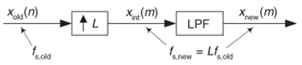
\includegraphics[width=0.5\linewidth]{graphics/Interpolation2}
	\caption{Interpolation.}
	\label{fig:Interpolation2}
\end{figure}

\subsection{Kombination af Interpolation og Decimation}
\begin{itemize}
	\item Samplerate konvertering; Interpolation med en faktor L efterfulgt af Decimation med en faktor M.
\end{itemize}

\begin{equation}
Sample\;rate\;conversion = \frac{L}{M}
\end{equation}

\begin{figure}[H]
	\centering
	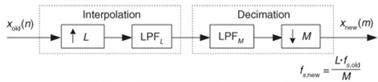
\includegraphics[width=0.4\linewidth]{graphics/multirate1}
	\caption{Kombination af interpolation/decimation.}
	\label{fig:multirate1}
\end{figure}

\begin{itemize}
	\item Interpolationsfiltret $LPF_L$ og decimeringsfiltret $LPF_M$ kan kombineres i et enkelt filter.
	\item Beregningsbyrden for at ændre sampleraten med $L/M$ er mindre når filterne kombineres end ved en individuel interpolation efterfulgt af en individuel decimation. 
\end{itemize}

\begin{figure}[H]
	\centering
	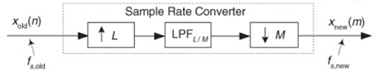
\includegraphics[width=0.4\linewidth]{graphics/multirate2}
	\caption{Anvendelse af et multirate filter.}
	\label{fig:multirate2}
\end{figure}

\begin{itemize}
	\item Dette kaldes for en sample rate converter.
	\begin{itemize}
		\item Hvis L > M har vi interpolation.
		\item Hvis M > L har vi decimering.	
	\end{itemize}
	\item Filteret $LPF_{L/M}$ kaldes ofte et multirate filter.
\end{itemize}

\begin{itemize}
	\item For at undgå aliasering skal filteret, $LPF_{L/M}$, dæmpe alle frekvenser der ligger over:
	\begin{itemize}
		\item $\frac{f_{s\,old}}{2}$
	\end{itemize}
	\item Eller hvis $LPF_{L/M}$ efter hvilen der er mindst:
	\begin{itemize}
		\item $\frac{f_{s\,old}}{2}(\frac{L}{M})$
	\end{itemize}
\end{itemize}








\newpage
\section{Differentiation og integration}

Differentiation er godt beskrevet for kontinuerte signaler, men differation for diskrete signaler er ikke veldefineret. Derfor bruges der forskellige modeller for tilnærmelsesvis beregning af de afledte derativer i digital signal behandling.

\subsection{First-difference differentiator}
\begin{itemize}
	\item Beregner differencen mellem hver sample. 
	\item Forstærker højfrekvente spektrale komponenter, har samme karakteristik som et højpas filter.
\end{itemize}

\begin{equation}
y_{Fd}(n) = x(n)-x(n-1) 
\end{equation}

\begin{figure}[H]
	\centering
	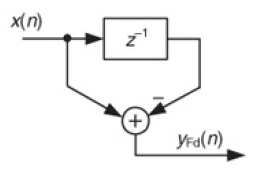
\includegraphics[width=0.3\linewidth]{graphics/first-difference-differentiator}
	\caption{First-difference differentiator.}
	\label{fig:first-difference-differentiator}
\end{figure}

\begin{figure}[H]
	\centering
	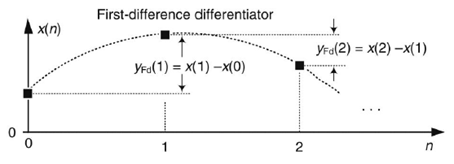
\includegraphics[width=0.6\linewidth]{graphics/first-difference-differentiator1}
	\caption{First-difference differentiator.}
	\label{fig:first-difference-differentiator1}
\end{figure}

\subsection{Central-difference differentiator}
\begin{itemize}
	\item Beregner den gennemsnitlige difference mellem hver 2. sample.
	\item Dæmper højfrekvente spektrale komponenter.
\end{itemize}

\begin{equation}
y_{Cd}(n) = \frac{x(n)-x(n-2)}{2}
\end{equation}

\begin{figure}[H]
	\centering
	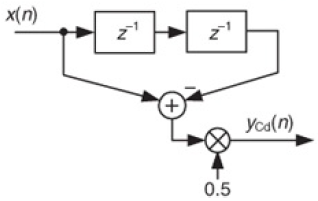
\includegraphics[width=0.3\linewidth]{graphics/central-difference-differentiator}
	\caption{Central-difference differentiator.}
	\label{fig:central-difference-differentiator}
\end{figure}

\begin{figure}[H]
	\centering
	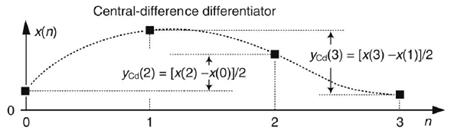
\includegraphics[width=0.6\linewidth]{graphics/central-difference-differentiator1}
	\caption{Central-difference differentiator.}
	\label{fig:central-difference-differentiator1}
\end{figure}

\begin{itemize}
	\item First-difference og Central-difference differentiators er kun præcise når input signalets båndbredde er lille i forhold til input signalets sample rate $f_s$. 
	\item Begge	differentiators har lineære fase respons og dermed en konstant tidsforsinkelse kaldet \textit{group delay}.
	\begin{itemize}
		\item First-difference differentiator har en delayline på $D = 1$ og dermed et group delay på \newline $G_{diff}= \frac{D}{2} = 1/2 = 0,5$ sample.
		\item Central-difference differentiator har en delayline på $D = 2$ og dermed et group delay på $G_{diff}= \frac{D}{2} = 2/2 = 1$ sample.
	\end{itemize}
\end{itemize}

\begin{figure}[H]
	\centering
	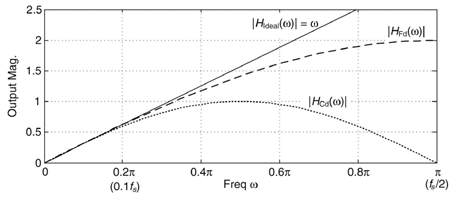
\includegraphics[width=0.6\linewidth]{graphics/frekvensrespons_diff}
	\caption{Frekvensrespons for simple differentiators.}
	\label{fig:frekvensrespons_diff}
\end{figure}

\subsection{Integration}
Integration er godt beskrevet for kontinuerte signaler, men integration for diskrete signaler er ikke veldefineret. Derfor bruges der forskellige modeller for tilnærmelsesvis kontinuert integration.

\paragraph{Rectangular Rule Integrator} udregner summen af de skraverede rektangler. Den nuværende sum $y_{Re}(n)$, er den forhenværende sum $y_{Re}(n-1)$ plus den nuværende input sample $x(n)$.

\begin{equation}
y{_Re}(n) = x(n)+y_{Re}(n-1)
\end{equation}

\begin{figure}[H]
	\centering
	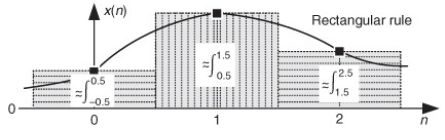
\includegraphics[width=0.6\linewidth]{graphics/rectangular_rule}
	\caption{Rectangular Rule Integrator.}
	\label{fig:rectangular_rule}
\end{figure}


\paragraph{Trapezoidal Rule Integrator} udregner summen af  $y_{Tr}(n)$ ved at beregne arealet ved gennemsnittet af $x(n) + x(n-1)$ i det skraverede areal til højre og addedere det med værdien for den forhenværende sum $y_{Tr}(n-1)$.
\begin{equation}
y_{Tr}(n) = 0.5 x(n)+ 0.5 x(n-1) + y_{Tr}(n-1)
\end{equation}

\begin{figure}[H]
	\centering
	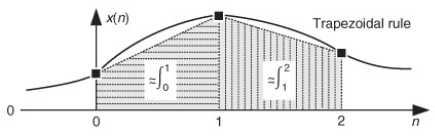
\includegraphics[width=0.6\linewidth]{graphics/trapezoidal_rule}
	\caption{Trapezoidal Rule Integrator.}
	\label{fig:trapezoidal_rule}
\end{figure}

\paragraph{Simpson's Rule Integrator} benytter tre samples til at beregne arealet under skraverede kurve.
\begin{equation}
y_{Si}(n) = \dfrac{x(n)+ 4x(n-1) x(n-2)}{3} + y_{Si}(n-2)
\end{equation}

\begin{figure}[H]
	\centering
	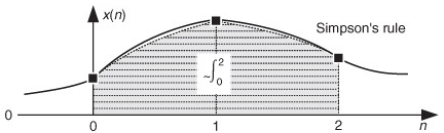
\includegraphics[width=0.6\linewidth]{graphics/simpsons_rule}
	\caption{Simpson's Rule Integrator.}
	\label{fig:simpsons_rule}
\end{figure}

\begin{itemize}
	\item Simple integrators er præcise ved lave frekvenser (når input signalets båndbredde er lille i forhold til input signalets sample rate $f_s$).
	\begin{itemize}
		\item Det er her hvor det er mest nødvendigt med høj præcision.
	\end{itemize}
	\item Ved højfrekvent støj scenarier skal Rectangular Rule eller Trapezoidal Rule integratorer anvendes, fordi de giver forbedret dæmpning af spektrale komponenter i nærheden af $\frac{f_s}{2}$.
\end{itemize}

\begin{figure}[H]
	\centering
	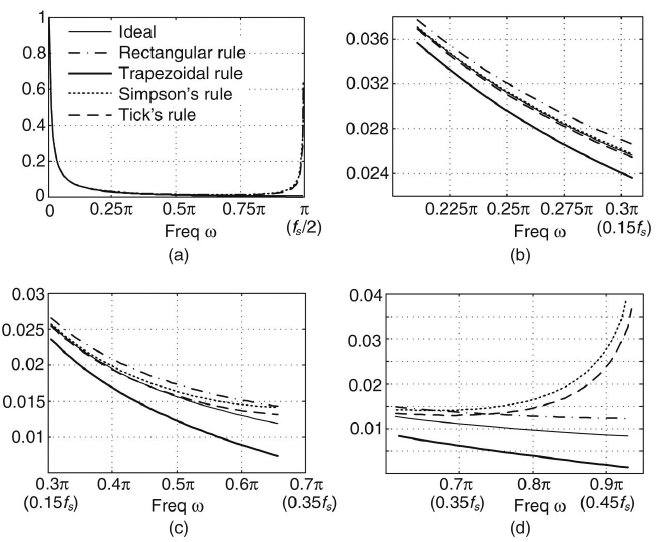
\includegraphics[width=0.6\linewidth]{graphics/integrators}
	\caption{Normaliseret frekvensrespons for fire integrators.}
	\label{fig:integrators}
\end{figure}


\newpage
\section{Stokastiske signaler, herunder middelværdi, varians, sandsynligheds-tæthedsfunktion og histogram}

\subsection{Stokastiske signaler}
\begin{itemize}
	\item Stokastisk ('tilfældig') signal.
	\begin{itemize}
		\item Modsat deterministisk ('forudsigelig') som kunne være en sinus-tone eller et firkant-signal.
		\item Kan ikke opskrive fast formel.
		\item Kan beskrive signalet med middelværdi, varians, sandsynlighedsfunktion.
	\end{itemize}
\end{itemize}

\subsection{Middelværdi}
\begin{itemize}
	\item DC niveau.
	\begin{itemize}
		\item Gennemsnittet af en sekvens af N samples er summen af disse samples divideret med N.
		\item $x_{ave}$ er den værdi som summen af forskellene mellem $x(n)$ og $x_{ave} = 0$. 
		\item Summen af sekvensen $d_{iff}(n) = x(n) - x_{ave} = 0$. 
		\item Lige meget værdi over som under gennemsnittet.
	\end{itemize}
\end{itemize}

\begin{equation}
x_{ave} = \frac{1}{N} \sum_{n=1}^{N}x(n)
\end{equation}

\begin{figure} [H]
	\centering
	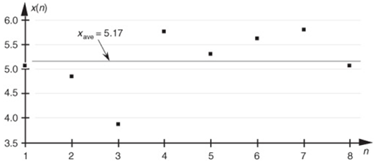
\includegraphics[width=0.6\linewidth]{graphics/x_ave}
	\caption{Gennemsnittet af en N lang sekvens. }
	\label{fig:x_ave}
\end{figure}

\subsection{Varians}
\begin{itemize}
	\item AC-middel-værdi.
\end{itemize}

\begin{equation}
{\sigma}^2 = \frac{1}{N} \sum_{n=0}^{N-1}(x(n)-x_{ave})^2
\end{equation}

\begin{figure} [H]
	\centering
	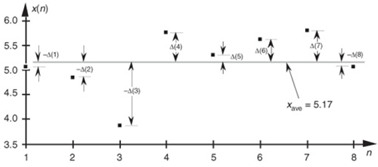
\includegraphics[width=0.6\linewidth]{graphics/var}
	\caption{Variansen hvor $\Delta(n) = x(n)-x_{ave}$.}
	\label{fig:var}
\end{figure}

\subsection{Standard afvigelse}
\begin{itemize}
	\item Standard afvigelsen svarer til RMS-værdien for en $DC=0$.
\end{itemize}

\begin{equation}
{\sigma} = {\sigma}^2
\end{equation}

\subsection{Sandsynligheds-tæthedsfunktion}
\begin{itemize}
	\item Normal fordeling.
	\item Kurven topper ved gennemsnittet $\si{\micro}_x$.
	\item Standardafvigelsen afgør faconen $\si{\micro}_x + \sigma$.
\end{itemize}

\begin{figure} [H]
	\centering
	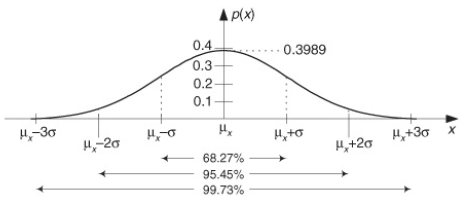
\includegraphics[width=0.6\linewidth]{graphics/pdf}
	\caption{Normalfordeling med gennemsnit = $\si{\micro}_x$.}
	\label{fig:pdf}
\end{figure}

\subsection{Histogram}
\begin{itemize}
	\item Histogrammets vertikale akse er antallet af gange, som en bestemt værdi indtræffer i signalet.
\end{itemize}

\begin{figure} [H]
	\centering
	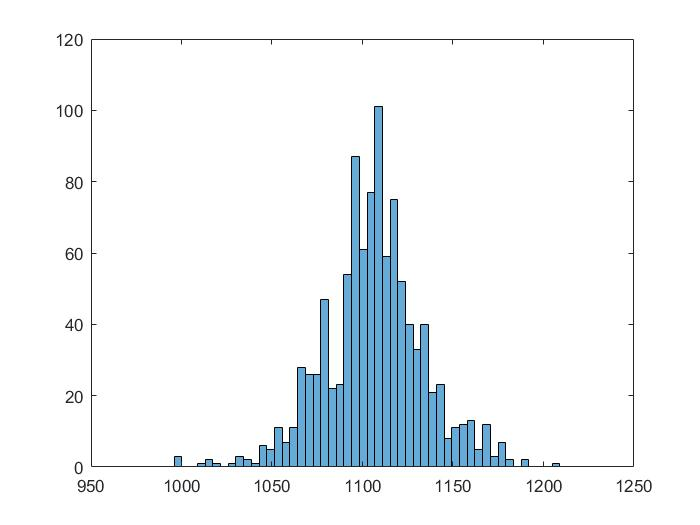
\includegraphics[width=0.4\linewidth]{graphics/histogram}
	\caption{Histogram.}
	\label{fig:histogram}
\end{figure}

\newpage
\section{Beregning af Signal-Noise Ratio i tids- og frekvens-domænet}

Signal-to-noise ratio er forholdet mellem det ønskede signal og det uønskede signal (støj).

\begin{equation}
SNR = \frac{P_{signal}}{P_{noise}}
\end{equation}

\paragraph{SNR i tidsdomænet}
\begin{itemize}
	\item Estimere SNR af et signal udfra signalets sampleværdier. 
	\item Middel-effekt.
\end{itemize}

\begin{equation}
P = \frac{1}{N} \sum_{n=0}^{N-1}x(n)^2
\end{equation}

\begin{itemize}
	\item AC middel-effekt.
\end{itemize}

\begin{equation}
P = {\sigma}^2 + x_{ave}^2
\end{equation}

\begin{itemize}
	\item SNR for AC udtrykkes ved variansen.
\end{itemize}

\begin{equation}
SNR = \frac{{\sigma}_s^2}{{\sigma}_n^2}
\end{equation}

\begin{itemize}
	\item I praksis kan et signal variere meget i effekt.
	\begin{itemize}
		\item Meget anvendt at bruge dB til at måle SNR.
	\end{itemize}
\end{itemize}

\begin{equation}
SNR_{dB} = 10 {\log}_{10}(SNR)
\end{equation}

\begin{itemize}
	\item Hvis rms er oplyst i stedet for effekt.
	\begin{itemize}
		\item Da der bruges en amplitude (volt eller ampere) i stedet for effekt benyttes $ 20 {\log}_{10}$ istedet for $ 10 {\log}_{10}$.
	\end{itemize}
\end{itemize}

\begin{equation}
x_{rms} = \sqrt{\frac{1}{N} \sum_{n=0}^{N-1}x(n)^2}
\end{equation}
­
\begin{equation}
SNR_{dB} = 20 {\log}_{10}\left(\frac{{x_{rms}}_{signal}}{{x_{rms}}_{noise}}\right)
\end{equation}


\paragraph{SNR i frekvensdomænet} kan groft estimateres baseret på signalets egenskaber i frekvensdomænet.

\begin{itemize}
	\item Der anvendes DFT på signalet i tidsdomænet og herefter fås de positive amplitudestørrelser $|X(m)|^2$.
	\item En threshold værdi fastsættes.
	\begin{itemize}
		\item Over threshold værdien er det ønskede signals amplitudestørrelse.
		\item Under treshold værdien er det uønskede støjsignals amplitudestørrelse.
	\end{itemize}
\end{itemize}

\begin{equation}
SNR=  \frac{sum\;of\;samples\;above\;threshold}{sum\;of\;samples\;below\;threshold}
\end{equation}

\begin{figure} [H]
	\centering
	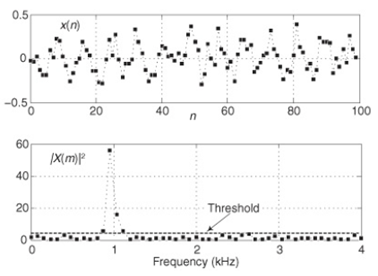
\includegraphics[width=0.6\linewidth]{graphics/snr}
	\caption{Øverst er støj afbildet i tidsdomænet. Nederst er støj afbildet i frekvensdomænet. }
	\label{fig:snr}
\end{figure}

\paragraph{Parseval's sætning} siger at energien bevares gennem Fourier’s transformation således at summen af kvadrerede samples i tidsdomænet er lig med summen af kvadrerede samples i frekvensdomænet.

\begin{equation}
\sum_{n=0}^{N-1}|x(n)|^2 = \frac{1}{N} \sum_{m=0}^{N-1}|X(m)|^2
\end{equation}


\newpage
\section{Midlingsfiltre}
Midlingsfiltre benyttes til at beregne en løbende middelværdi for et signal. 

\begin{figure} [H]
	\centering
	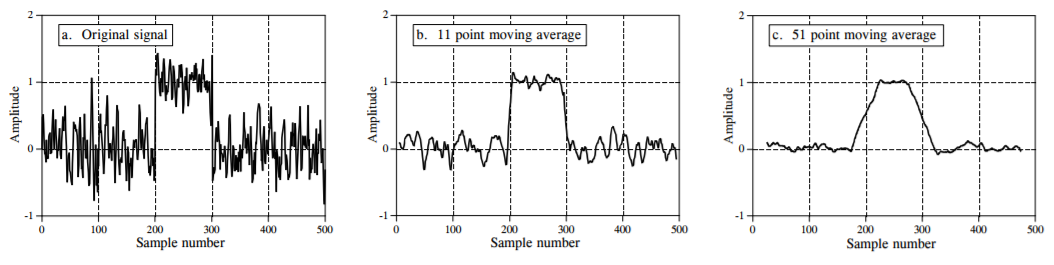
\includegraphics[width=\linewidth]{graphics/ma}
	\caption{Signal før og efter det er filtreret med midlingsfilter.}
	\label{fig:ma}
\end{figure}

\subsection{Ikke-rekursiv}
\begin{itemize}
	\item FIR filter med N antal filterkoefficienter. 
	\item Har $N-1$ delay elementer.
\end{itemize}

\begin{equation}
y(n)=\frac{1}{N}(x(n)+x(n-1)+x(n-2)+x(n-N+1))
\end{equation}

\begin{figure} [H]
	\centering
	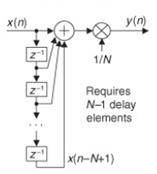
\includegraphics[width=0.25\linewidth]{graphics/nonrecursic}
	\caption{Ikke Rekursiv midlingsfilter.}
	\label{fig:nonrecursic}
\end{figure}

\subsection{Rekursiv}
\begin{itemize}
	\item Mindre beregningstung, da den kun kræver 2 adderinger pr. output sample uanset antallet af delays.
	\item Har $N$ delay elementer, altså et ekstra delay iforhold til ikke-rekursiv midlingsfilter. 
\end{itemize}

\begin{equation}
y(n)=\frac{1}{N}(x(n)-x(n-N))+y(n-1)
\end{equation}

\begin{figure} [H]
	\centering
	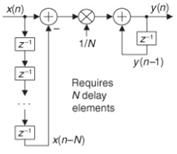
\includegraphics[width=0.3\linewidth]{graphics/recursic}
	\caption{Rekursiv midlingsfilter.}
	\label{fig:recursic}
\end{figure}

\subsubsection{Frekvensrespons}
\begin{itemize}
	\item Ikke-rekursiv og rekursiv midlingsfiltre har akkurat samme frekvensrespons. 
	\item "The roll-off" er meget langsom og stopbåndets dæmpning er ringe.
	\item \textit{Remember, good performance in the time domain results in poor performance
		in the frequency domain, and vice versa.}\footnote{The Scientist and Engineer's Guide to Digital Signal Processing Moving Average Filters, Chapter 15, Page 180.}
	\begin{itemize}
		\item Midlingsfilteret er et fantastisk midlingsfilter i tidsdomænet, men en elendig lavpas filter i frekvensdomænet.
	\end{itemize}
\end{itemize}


\begin{figure} [H]
	\centering
	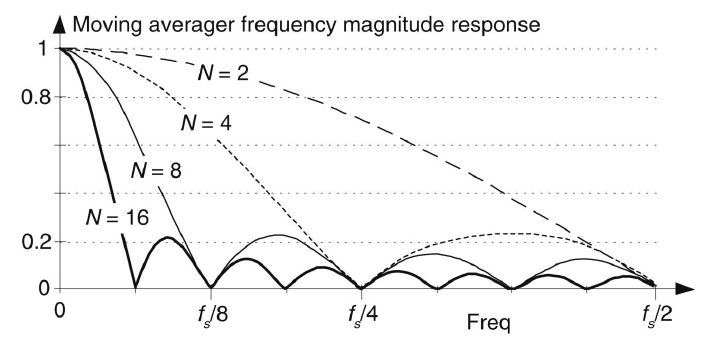
\includegraphics[width=0.6\linewidth]{graphics/ma_freqresponse}
	\caption{Frekvensrespons for et midlingsfilter med N antal filterkoefficienter.}
	\label{fig:ma_freqresponse}
\end{figure}

\subsection{Eksponentielt midlingsfilter}
\begin{itemize}
	\item Nyeste samples får størst vægt.
	\item Reagerer hurtigere på ændringer i input ifht. almindelig midlingsfilter.
	\item Faktoren $0<\si{\alpha}<1$ bestemmer hvor meget vægt tidligere output værdier skal have for nye output værdier.
	\begin{itemize}
		\item Hvis $\si{\alpha}=1$ ignoreres tidligere output værdier, da nye output værdier reagerer med det samme på nye input værdier samtidig giver det ingen dæmpning.
	\end{itemize}
\end{itemize}

\begin{figure} [H]
	\centering
	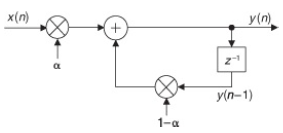
\includegraphics[width=0.4\linewidth]{graphics/exponentieltfilter}
	\caption{Eksponentielt midlingsfilter.}
	\label{fig:exponentieltfilter}
\end{figure}

\subsubsection{Støjreduktion}
\begin{itemize}
	\item En mindre \si{\alpha} værdi giver en bedre støjreduktion men midlingsfilterets output tager samtidig længere tid om at reagere og stabilisere sig. 
\end{itemize}

\begin{figure} [H]
	\centering
	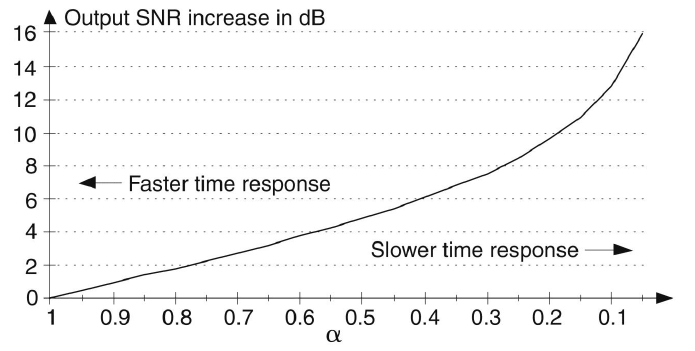
\includegraphics[width=0.6\linewidth]{graphics/exp_snr}
	\caption{Eksponentielt midlingsfilterets SNR som en funktion af faktoren \si{\alpha}.}
	\label{fig:exp_snr}
\end{figure}

\begin{itemize}
	\item Midlingsfilterets SNR kan regnes herved.
\end{itemize}

\begin{equation}
SNR_{exp(dB)} = 10 \log_{10}\left(\dfrac{\si{\alpha}}{2-\si{\alpha}}\right)
\end{equation}

\newpage
\section{Auto- og kryds-korrelation}
\subsection{Foldning}
Foldning er en matematisk måde at kombinere to signaler til at danne et tredje signal.
\subsubsection{Delta Funktion og Impuls Respons}
\begin{itemize}
	\item Delta-funktionen $\delta[n]$ er en normaliseret impuls.
	\item Alle dens samples har en værdi på 0, bortset fra samplenummer 0, som har en værdi på 1.
	\item Impuls responset $h[n]$ for et lineært system er outputtet fra systemet, når inputtet er en delta-funktion.
\end{itemize}

\begin{figure} [H]
	\centering
	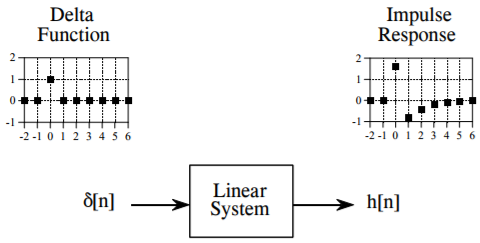
\includegraphics[width=0.6\linewidth]{graphics/deltafunction_impulseresponse}
	\caption{Definition af delta funktionen og impuls responset.}
	\label{fig:deltafunction_impulseresponse}
\end{figure}

\begin{itemize}
	\item Inputsignalet foldet med systemets impuls respons er svarende til outputsignalet.
	\item Hvis x[n] er et signal med N antal samples fra 0
	til N-1, og h[n] er et signal med M antal samples fra 0 til M-1, bliver foldningen af de to signaler:  $y(n) = x(n) \circledast y(n)$, et signal med $N+M-1$ antal samples fra 0 til $N+M-2$.
\end{itemize}

\begin{equation}
y(n) = \sum_{k=0}^{M-1} h(k) \cdot x(n-k) = h(n) \circledast x(n)
\end{equation}

\begin{itemize}
	\item Inputsignalet x(k) flippes rundt så dette placerer
	sample 0 til højre og efterfølgende opadgående samples til venstre.
	\begin{itemize}
		\item x(k) bliver herved til x(-k).
	\end{itemize}
	\item Alle produkter af h(k) og x(0-k) for alle k-værdier summeres og herved fås y(0).
	\item x(-k) shiftes en sample til højre.
	\item  Alle produkter af h(k) og x(1-k) for alle k-værdier summeres og herved fås y(1).
	\item Der shiftes og summeres indtil der ikke er overlap mellem h(k) og x(n-k).
\end{itemize}

\begin{figure}[H]
	\centering
	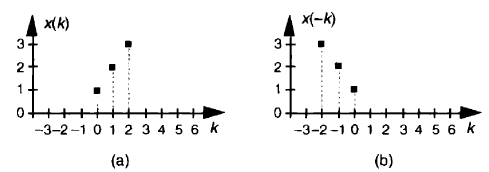
\includegraphics[width=0.6\linewidth]{graphics/convolution}
	\caption{(a) sekvensen $x(k)$; (b) spejling af sekvensen $x(k)$ omkring $k = 0$.}
	\label{fig:convolution}
\end{figure}

\textbf{Foldnings‐teorem I} betyder at foldning af to signaler i tidsdomænet er det samme som multiplikation af to signaler i frekvensdomænet.

\begin{equation}
h(n) \circledast x(n) \Leftrightarrow H(e^{j\omega}) \cdot X(e^{j\omega})
\end{equation}

\textbf{Foldnings-teorem II} betyder at foldning af to signaler i frekvensdomænet er det samme som multiplikation af to signaler i tidsdomænet. 

\begin{equation}
h(n) \cdot x(n) \Leftrightarrow H(e^{j\omega}) \circledast X(e^{j\omega})
\end{equation}

\subsection{Krydskorrelation}
Korrelation mellem 2 signaler.
Kan bruges til at finde periodicitet i et signal, signaldetektion eller system identifikation

\begin{itemize}
	\item Amplituden af hver sample i krydskorrelationssignalet er mål for hvor meget det signal der er optaget lignet det oprindelige target signal.
	\item r(n) er derfor et mål for, hvor meget et signal ligner et andet signal - tidsforskudt med n.
\end{itemize}
\begin{equation}
r(n) = \sum_{k=-\infty}^{\infty} h(k) \cdot x(n+k) = h(n) \circledast x(-n)
\end{equation}

\begin{figure}[H]
	\centering
	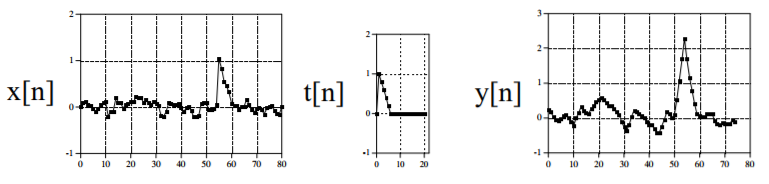
\includegraphics[width=0.8\linewidth]{graphics/crosscorrelation}
	\caption{y(n) er krydskorrelationen mellem x(n) og t(n).}
	\label{fig:crosscorrelation}
\end{figure}

\subsection{Autokorrelation}
Korrelation af signal med sig selv tidsforskudt.

\begin{equation}
r(n) = \sum_{k=-\infty}^{\infty} x(k) \cdot x(n+k) = x(n) \circledast x(-n)
\end{equation}

\newpage
\section{CASE projekt 1 – FSK transmission}
\subsection{Opgavebeskrivelse}
\begin{itemize}
	\item Lave et kommunikationssystem imellem to enheder, hvor hver enhed har en mikrofon og en højttaler. 
	\item Der benyttes en hørbar lyd som generes som et lydsignal-array.
	\item Bit rate, båndbredde og betydning af signal-støj-forhold.
\end{itemize}

\subsection{Analyse af lydsignal}
\begin{itemize}
	\item Analyse af hvilke karakterer, som svarer til hvilke frekvenser. 
	\item Signalet analyseres vha. Short-Time Fourier Transform – dvs. med spektrogram-plot.
	\begin{itemize}
		\item Et smalt vindue giver en god opløsning i tid, men giver en dårlig opløsning i frekvens.
		\item Et bredt vindue giver en god opløsning i frekvens, men en dårlig opløsning i tid.
	\end{itemize}
\end{itemize}

\begin{figure}[H]
	\centering
	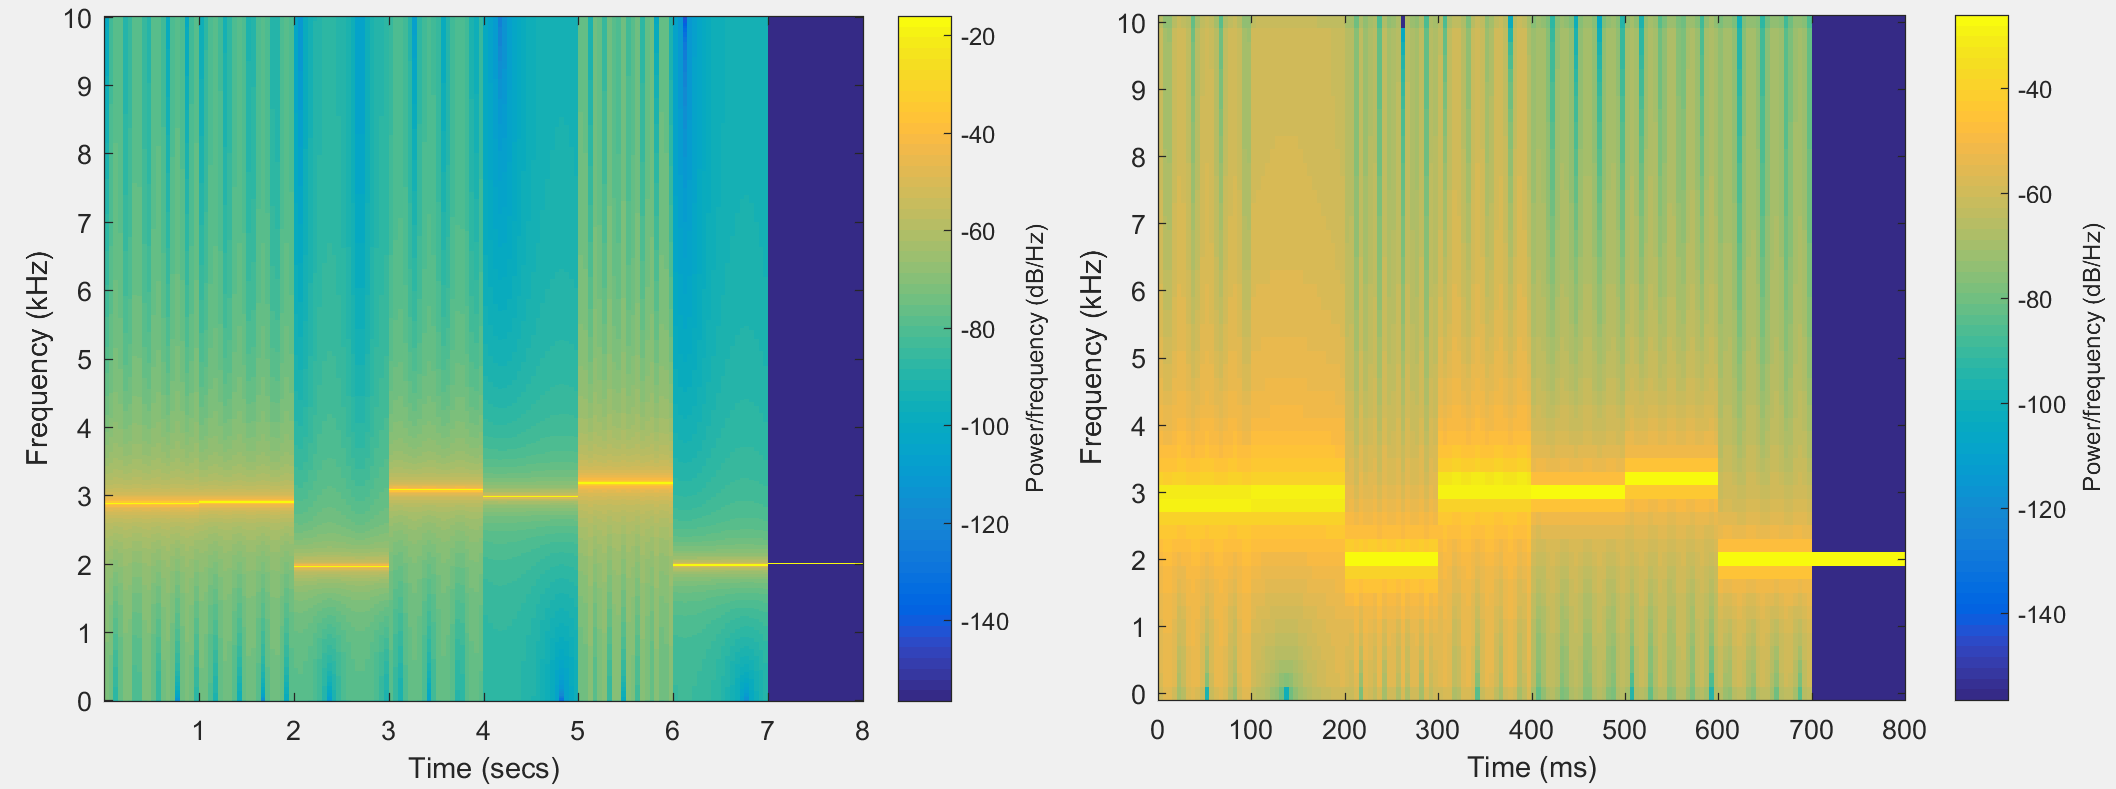
\includegraphics[width=\linewidth]{graphics/case1_2}
	\caption{V: God opløsning i frekvens og dårlig opløsning i tid. H: God opløsning i tid og dårlig opløsning i frekvens.}
	\label{fig:case1_2}
\end{figure}

\subsection{Dekodning}
\begin{itemize}
	\item Frekvensbåndet der arbejdes indenfor er kendt og dermed den laveste frekvens og højeste frekvens. 
	\item Længden af hvert symbol er også kendt.
	\item Antallet af symboler der er blevet sendt findes ved hjælp af samplefrekvensen samt længden på det modtagne signal.
\end{itemize}

\begin{equation}
\Delta R = \frac{f_s}{N}
\end{equation}

\subsection{Signal-støj-forhold}
\begin{itemize}
	\item Jo større distance mellem enhederne, jo mindre bliver effekten af signalet fra højtalerne, og jo mere består det samlede signal af støj.
	\begin{itemize}
		\item Signalet blev optaget ved 4 forskellige distancer (\SI{0}{\meter}, \SI{0}{\meter}, \SI{0}{\meter} og \SI{0}{\meter}).
	\end{itemize}
\end{itemize}

\begin{equation}
SNR = \frac{P_{signal}}{P_{noise}}
\end{equation}

\paragraph{SNR i tidsdomænet}
\begin{itemize}
	\item Estimere SNR af et signal udfra signalets sampleværdier. 
	\item Middel-effekt.
\end{itemize}

\begin{equation}
P = \frac{1}{N} \sum_{n=0}^{N-1}x(n)^2
\end{equation}

\paragraph{SNR i frekvensdomænet} kan groft estimateres baseret på signalets egenskaber i frekvensdomænet.

\begin{itemize}
	\item Der anvendes DFT på signalet i tidsdomænet og herefter fås de positive amplitudestørrelser $|X(m)|^2$.
	\item En threshold værdi fastsættes.
	\begin{itemize}
		\item Over threshold værdien er det ønskede signals amplitudestørrelse.
		\item Under treshold værdien er det uønskede støjsignals amplitudestørrelse.
	\end{itemize}
\end{itemize}

\begin{equation}
SNR=  \frac{sum\;of\;samples\;above\;threshold}{sum\;of\;samples\;below\;threshold}
\end{equation}

\subsection{Bit rate}
\begin{itemize}
	\item Ved en enkelt tone kan der aflæses fint med en symbollængde på \SI{0,1}{\second}
	\item  Hvis der er to frekvenser tæt på hinanden skal der bruges en symbollængde på \SI{0,5}{\second}.
	\item Der kan anvendes zero-padding til at få den korrekte amplitude.
\end{itemize}

\newpage
\section{CASE projekt 2 – Audio filter}
\subsection{Opgavebeskrivelse}
\begin{itemize}
	\item Analysere støjfyldt lydsignal og undersøge hvilken frekvens som ønskes fjernet.
	\item Designe IIR filter ved placering af poler/nuller.
	\item Implementere IIR filter på Blackfin processor.
\end{itemize}

\subsection{Analyse af lydsignal}
\begin{itemize}
	\item Frekvensanalyse med DFT af lydfil hvorved støjsignal findes.
	\item  På et spektrogram kan den gennemgående støj ses som en gul streg ved frekvensen \SI{785}{\hertz}.
\end{itemize}

\begin{figure}[H]
	\centering
	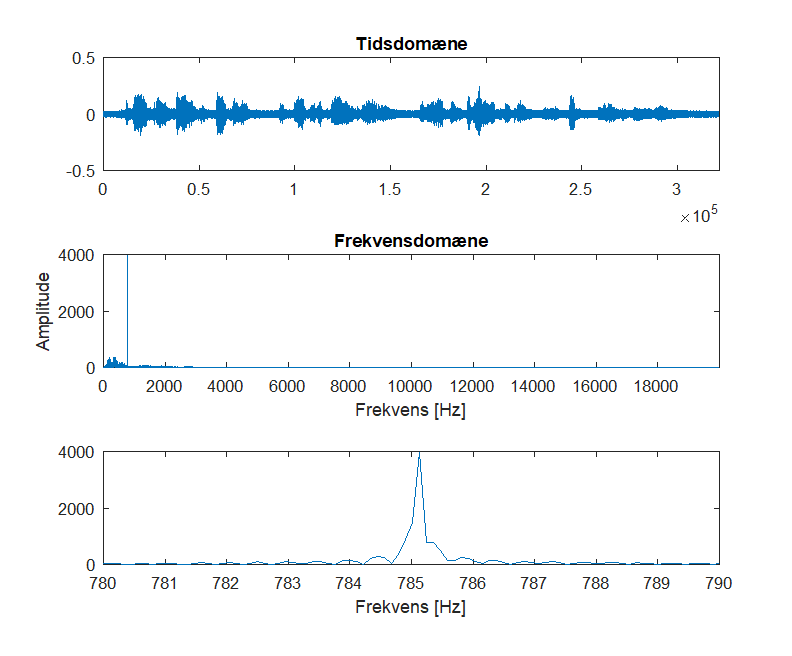
\includegraphics[width=0.6\linewidth]{graphics/case2_1}
	\caption{Signalet i tidsdomænet og efterfølgende DFT af signalet.}
	\label{fig:case2_1}
\end{figure}

\begin{figure}[H]
	\centering
	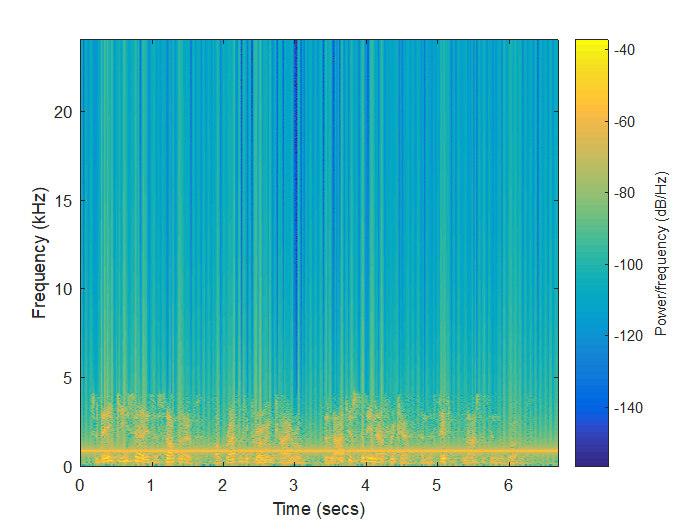
\includegraphics[width=0.6\linewidth]{graphics/case2_2}
	\caption{Spektrogramanalyse af signalet.}
	\label{fig:case2_2}
\end{figure}

\subsection{Design af IIR filter}
\begin{itemize}
	\item Poler danner peaks.
	\begin{itemize}
		\item Har betydning for hvor meget frekvenserne bliver forstærket, hvis den placeres på enhedscirklen forstærkes frekvenserne uendeligt meget.
	\end{itemize}
	\item Nulpunkter danner dyk.
	\begin{itemize}
		\item Har betydning for hvor meget frekvenserne bliver dæmpet, hvis den placeres på enhedscirklen dæmpes frekvenserne uendeligt meget.
	\end{itemize}
	\item Stabilitet.
	\begin{itemize}
		\item Hvis alle poler er placeret inde i enhedscirklen vil filteret være stabilt.
		\item Polen kan ophæves ved at have et nulpunkt med præcis samme afstand fra (0,0) og dermed samme længde.
		\item Poler/nulpunkter placeret i (0,0) påvirker ikke filterets frekvens respons. 
	\end{itemize}
\end{itemize}

\begin{figure}[H]
	\centering
	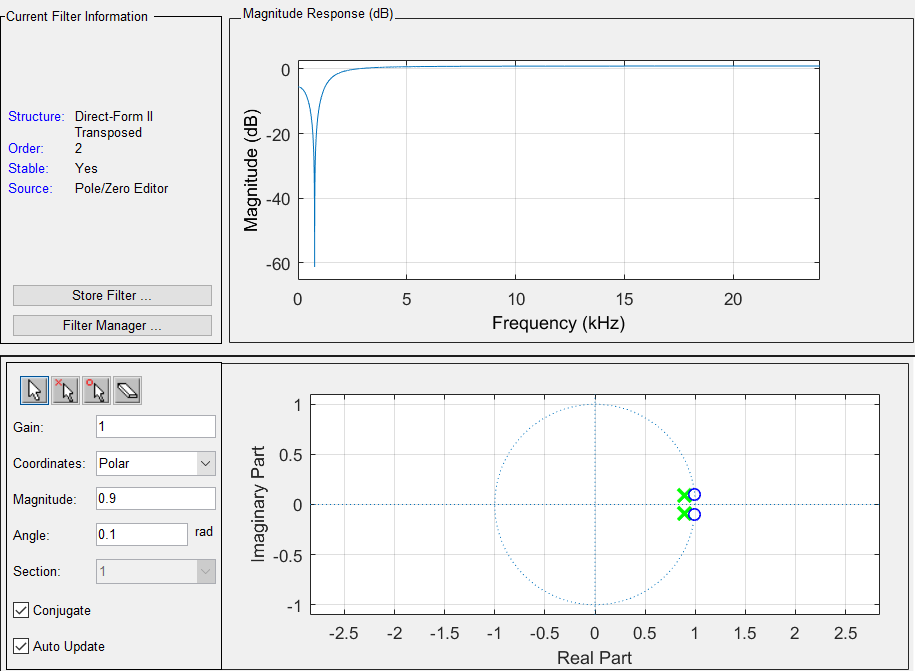
\includegraphics[width=0.6\linewidth]{graphics/case2_3}
	\caption{IIR filter poler/nulpunkter og frekvens respons.}
	\label{fig:case2_3}
\end{figure}


\begin{itemize}
	\item Et 2. ordens IIR notch filter designes ved at placere poler og nulpunkter i z-domænet.
	\item Nulpunkter/poler har en radius og vinkel da de er komplekse tal.
	\begin{itemize}
		\item $r$ er nul-radius og $\omega$ er nul-vinkel.
		\item Nul-radius sættes til 1 og pol-radius sættes til 0,9 da det et skarpt filter ønskes.
	\end{itemize}
\end{itemize}

\begin{equation}
z_0 = r e^{j\omega} = e^{j\omega}
\end{equation}

\begin{equation}
p_0 = r e^{j\omega} = 0,9 e^{j\omega}
\end{equation}

\begin{itemize}
	\item Vinklen af de to nulpunkter og to poler beregnes (kompleks konjugerede).
\end{itemize}

\begin{equation}
\omega = 2\pi \frac{f}{f_s} = 2\pi \frac{\SI{785}{\hertz}}{\SI{48}{\kilo\hertz}} = 0,1028
\end{equation}

\newpage
\begin{itemize}
	\item Overførelsesfunktionen H(z) i z-domænet opstilles ud fra poler/nulpunkter.
\end{itemize}

{\setlength\parindent{24pt}
\begin{tabular}{l}
	$z_0 =  e^{j0,1028}$ \\ 

	$\overline{z_0} =  e^{-j0,1028}$ \\ 
	
	$p_0 = 0,9 e^{j0,1028}$ \\ 
	
	$ \overline{p_0} = 0,9 e^{-j0,1028}$ \\ 
\end{tabular}} 

\begin{equation}
H(z) = \frac{Y(z)}{X(z)} = G \frac{(z - z_0)(z-\overline{z_0})}{(z - p_0)(z-\overline{p_0})} = G \frac{(z - e^{j0,1028})(z - e^{-j0,1028})}{(z - 0,9\cdot  e^{j0,1028})(z-0,9\cdot e^{-j0,1028})}
\end{equation}

\begin{figure}[H]
	\centering
	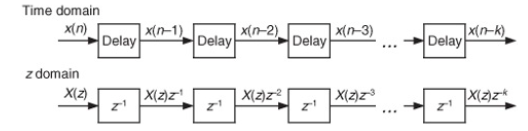
\includegraphics[width=0.6\linewidth]{graphics/z_domain_delay}
	\caption{Tids- og z-domæne delay.}
	\label{fig:z_domain_delay}
\end{figure}

\begin{itemize}
	\item Overførselsfunktionen H(z) skrives om således at polynomierne er opløftet negativt.
\end{itemize}

\begin{equation}
H(z) = \frac{z^2 - 1,99z + 0,99}{z^2 - 1,79z + 0,81} \cdot \frac{z^{-2}}{z^{-2}} \longrightarrow \frac{1 - 1,99z^{-1} + 0,99z^{-2}}{1 - 1,79z^{-1} + 0,81z^{-2}}
\end{equation}

\begin{itemize}
	\item Brøkerne kan skrives ud.
\end{itemize}

\begin{equation}
Y(z)(1-1,79z^{-1}+0,81z^{-2}) = X(z)(1-1,99z^{-1}+0,99 z^{-2})
\end{equation}

\begin{itemize}
	\item Differensligningen kan opstilles ved at anvende invers z-transformation.
\end{itemize}

\begin{equation}
y(n)-1,79y(n-1)+0,81y(n-2)=x(n)-1,99x(n-1)+0,99x(n-2)
\end{equation}

\begin{equation}
y(n)=1x(n)-1,99x(n-1)+0,99x(n-2)+1,79y(n-1)-0,81y(n-2)
\end{equation}

\begin{itemize}
	\item Filterkoefficienterne bliver dermed.
\end{itemize}

{\setlength\parindent{24pt}
\begin{tabular}{l}
	$b_0 = 1$ \\ 
	
	$b_1 = -1,99$ \\ 
	
	$b_2 = 0,99$ \\ 
	
	$a_0 = 1,79$ \\ 
	
	$a_1 = -0,81$ \\
\end{tabular}}

\subsection{Implementation på Blackfin processor}
\begin{itemize}
	\item Datatypen ”short” anvendes til variablene, da der arbejdes på en fixed-point processor.
	\item Bitmanipulation (1 << 14)
	\begin{itemize}
		\item  Bit 1 er signbit som afgør om det er positiv eller negativ talværdi. 
		\item Bit 2 er fixed-point binary som placerer kommaet det samme sted.
	\end{itemize}
	\item Der bitshiftes dermed 14 pladser til venstre for at placere filterkoefficienter som MSB lige efter signbit og fixed-point bit.
\end{itemize}

\newpage
\section{CASE projekt 3 – Vejecelle}
\subsection{Opgavebeskrivelse}
\begin{itemize}
	\item Analysere og forbedre dataene fra en støjfyldt måling på en vejecelle.
	\item Der designes og implementeres forskellige midlingsfiltre i Matlab for at fjerne støj.
\end{itemize}

\begin{figure}[H]
	\centering
	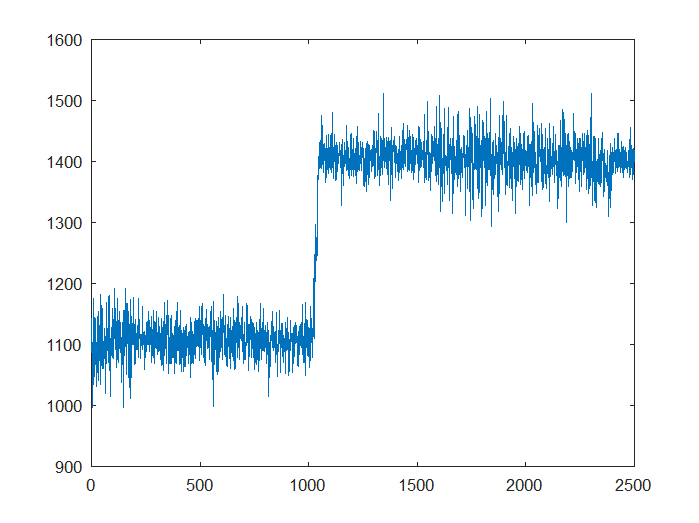
\includegraphics[width=0.3\linewidth]{graphics/case3_1}
	\caption{Vejecelle måling med \SI{1}{\kilogram} belastning og  uden belastning.}
	\label{fig:case3_1}
\end{figure}

\subsection{Data analyse}
\begin{itemize}
	\item Den første del af signalet er med \SI{1}{\kilogram} belastning og næste del er uden belastning. 
	\item  Signalet deles derfor op for at kunne udregne middelværdi, spredning og varians af de to forskellige målinger.
\end{itemize} 

\paragraph{Middelværdi} er gennemsnittet af sekvensen på N samples er summen af disse samples divideret med N. Der er lige meget værdi over som under gennemsnittet.

\begin{equation}
x_{ave} = \frac{1}{N} \sum_{n=1}^{N}x(n) \approx 1100  \ldots 1400
\end{equation}

\paragraph{Varians} er AC-middel-værdien.

\begin{equation}
{\sigma}^2 = \frac{1}{N} \sum_{n=0}^{N-1}(x(n)-x_{ave})^2 \approx 772  \ldots 794
\end{equation}

\paragraph{Standard afvigelse} svarer til RMS-værdien for en $DC=0$. Standard afvigelsen kaldes også for spredningen. 

\begin{equation}
{\sigma} = {\sigma}^2 \approx 27  \ldots 28
\end{equation}

\begin{itemize}
	\item Variansen og spredningen for de to målinger er cirka den samme. 
	\begin{itemize}
		\item Forventeligt da det kun er DC værdien der burde ændres.
	\end{itemize}
\end{itemize}

\begin{figure}[H]
	\centering
	\includegraphics[width=0.42\linewidth]{graphics/case3_2}
	\caption{Histogram af de to signalniveauer normal fordelt rundt om deres middelværdi.}
	\label{fig:case3_2}
\end{figure}

\subsection{Midlingsfiltre}
\paragraph{Ikke-rekursiv midlingsfilter}
\begin{itemize}
	\item Mindre beregningstung, da den kun kræver 2 adderinger pr. output sample uanset antallet af delays.
	\item Har $N$ delay elementer, altså et ekstra delay iforhold til ikke-rekursiv midlingsfilter. 
\end{itemize}

\begin{equation}
y(n)=\frac{1}{N}(x(n)-x(n-N))+y(n-1)
\end{equation}

\begin{figure} [H]
	\centering
	\includegraphics[width=0.3\linewidth]{graphics/recursic}
	\caption{Rekursiv midlingsfilter.}
	\label{fig:recursic}
\end{figure}

\begin{figure}[H]
	\centering
	\includegraphics[width=0.65\linewidth]{graphics/case3_3}
	\caption{Vejecelle måling med \SI{1}{\kilogram} belastning og  uden belastning med et 10. og 100. ordens midlingsfilter.}
	\label{fig:case3_3}
\end{figure}

\begin{itemize}
	\item Midlingsfilteret gør at der kommer en indsvingningstid. \begin{itemize}
		\item Ved et 10. ordens filter nås DC værdien efter cirka 10 samples.
		\item Ved et 100. ordens filter nås DC værdien efter cirka 100 samples.
	\end{itemize}
\end{itemize}

\begin{figure}[H]
	\centering
	\includegraphics[width=0.6\linewidth]{graphics/case3_4}
	\caption{Histogram af de to signalniveauer normal fordelt efter midlingsfilteret. Dataen er mere samlet.}
	\label{fig:case3_4}
\end{figure}

\paragraph{Eksponentielt midlingsfilter}
\begin{itemize}
	\item Nyeste samples får størst vægt.
	\item Reagerer hurtigere på ændringer i input ifht. almindelig midlingsfilter.
	\item Faktoren $0<\si{\alpha}<1$ bestemmer hvor meget vægt tidligere output værdier skal have for nye output værdier.
	\begin{itemize}
		\item Hvis $\si{\alpha}=1$ giver det ingen dæmpning og samtidig ignoreres tidligere output værdier, da nye output værdier reagerer med det samme på nye input værdier.
	\end{itemize}
\end{itemize}

\begin{figure} [H]
	\centering
	\includegraphics[width=0.4\linewidth]{graphics/exponentieltfilter}
	\caption{Eksponentielt midlingsfilter.}
	\label{fig:exponentieltfilter}
\end{figure}


\begin{figure}[H]
	\centering
	\includegraphics[width=0.6\linewidth]{graphics/case3_5}
	\caption{Vejecelle måling med \SI{1}{\kilogram} belastning og  uden belastning med et 10. og 100. ordens eksponentielt midlingsfilter.}
	\label{fig:case3_5}
\end{figure}


\newpage
\section{CASE projekt 4 - Sonar}
\subsection{Opgavebeskrivelse}
\begin{itemize}
	\item Afstandsbestemmelse ved et udsende et akustisk signal.
	\item Systemet vil afspille og optage ekko-signalet på Blackfin kittet.
	\item Afstanden findes ved hjælp af krydskorrelation. 
\end{itemize}
	
\subsection{Signal generation}
\begin{itemize}
	\item Krav til signalet er at samplefrekvensen er \SI{48}{\kilo\hertz}, da det er denne som Blackfin kittet arbejder med. Vi vælger \SI{50}{\milli\second} og derfor får vi en arraystørrelse på 2400 samples.
	\item Et unikt signal ønskes, hvorfor et sweep eller hvid støj er bedre end et sinus signal. 
	\begin{itemize}
		\item Et sinus signal er kontinuert og da den gentager sig selv er det et problem da vi med korrelation leder efter gentagelser.
	\end{itemize} 
	\item Længden af signalet skal sørge for at være langt nok til at optage både når signalet sendes afsted og indtil det er kommet tilbage. 
	\item Præcisionen af målingen er ca. \SI{7}{\milli\meter} per sample.
\end{itemize} 
\begin{equation}
 \frac{\SI{340}{\meter\per\second}}{\SI{48}{\kilo\hertz}} \approx \SI{7}{\milli\meter}
\end{equation}
\begin{itemize}
	\item Systemet skal kunne måle afstande op til \SI{10}{\meter}. Dette giver en forventning om at ekkoet skal rejse \SI{20}{\meter}. Det vil tage ekkoet \SI{59}{\milli\second} at rejse 20 meter.
\end{itemize}
\begin{equation}
\frac{\SI{20}{\meter}}{\SI{340}{\meter\per\second}} \approx \SI{59}{\milli\second}
\end{equation}
\begin{itemize}
	\item Antal samples der er brug for til at optage afspilningen er $F_s \cdot T + 2400 \cdot 2 \approx 7600$.
	\item Array størrelsen bliver hermed $2^{13} = 8192$.
	\item Optagetiden er herved \SI{160}{\milli\second}.
\end{itemize}
\begin{equation}
\frac{N}{F_s} = \frac{7600}{\SI{48}{\kilo\hertz}} \approx \SI{160}{\milli\second}
\end{equation}

\subsection{Signal analyse}
\begin{itemize}
	\item Krydskorrelation anvendes mellem det udsendte signal og de optagede signaler for at finde tidsforskydningen.
	\item Distancen kan beregnes ved den sample hvor der opstår peak i krydskorrelationen.
\end{itemize}

\begin{equation}
Distance = Sample\cdot \SI{340}{\meter\per\second} \cdot \frac{1}{\SI{48}{\kilo\hertz}} \cdot 0.5
\end{equation}
\begin{table} [H]
	\centering
\begin{tabular}{|c|c|c|}
	\hline 
	Afstand målt [m] & Afstand udregnet [m] & Difference [cm] \\ 
	\hline 
	1 & 0,935 & 6,5 \\ 
	\hline 
	1,5 & 1,678 & 17,8 \\ 
	\hline 
	2 & 2,001 & 0,1 \\ 
	\hline 
	3 & 3,184 & 18,4 \\ 
	\hline 
	4,5 & 4,388 & 11,2 \\ 
	\hline 
\end{tabular} 
\caption{Resultater af analyse.}
\end{table}

\begin{figure}[H]
	\centering
	\includegraphics[width=0.54\linewidth]{graphics/case4_opg4_1}
	\caption{Stem af krydskorrelation for \SI{1}{\meter}.}
	\label{fig:case4_opg4_1}
\end{figure}

\begin{figure}[H]
	\centering
	\includegraphics[width=0.54\linewidth]{graphics/case4_opg4_2}
	\caption{Stem af krydskorrelation for \SI{2}{\meter}.}
	\label{fig:case4_opg4_2}
\end{figure}

\begin{figure}[H]
	\centering
	\includegraphics[width=0.54\linewidth]{graphics/case4_opg3}
	\caption{Højtaleren er tæt på mikrofonen hvorfor signalet er meget kraftigere i starten af optagelsen.}
	\label{fig:case4_opg3}
\end{figure}


\end{document}